\chapter{The LHC and The CMS Experiment}

\section{The LHC}
The Large Hadron Collider(LHC) is the largest and most powerful superconducting hadron accelerator and collider. The LHC was installed in an existing 26.7 km tunnel that was constructed for LEP machine between 1984 and 1989. The tunnel of LHC has 8 straight sections and 8 arcs, and locates between 45m and 170m below the surface. The LHC host 4 experiments currently: CMS(Point 5), ATLAS(Point 1), ALICE(Point 2) and LCHb(Point 8).
\subsection{LHC: Performance and Main machine layout}

\begin{figure}[htbp]
 \begin{center}
  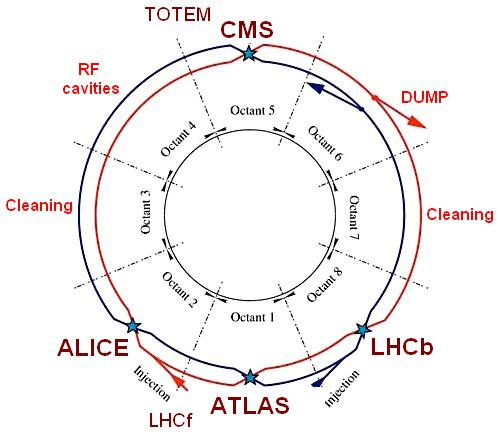
\includegraphics[width=0.8\textwidth]{figures/c3/c3_lhc_latticelayout.jpg}
 \end{center}
 \caption{abcf}
 \label{fig:c3lhclayout}
\end{figure}
Performance, eq, lumi, xsection. Lumi equation from lhc parameter.
Main machine layout: 2 beam with 2 rings, 8 long straight sections and 8 arcs.

\begin{equation}
 L = \frac{N^{2}_{b}n_{b}f_{rev}\gamma_{r}}{4\pi \varepsilon_{n}\beta *}F \;
 \label{eq:c3lhclumi}
\end{equation}

\begin{equation}
 F = (1+\frac{\theta_{c}\sigma_{c}}{2\sigma *})^{-1/2} \;
 \label{eq:c3lhcgeof}
\end{equation}

\subsection{LHC: From operation point of view}
The LHC is a extremely complex machine and it is almost impossible to grasp all details. However, the LHC is provide a summary of status for the operational activities, which are very useful in the detector operation.
\subsubsection{Acclerator Mode}
The accelerator mode provides a summary status of the LHC machine.The detector system(eg. CMS) need to make daily operational decision accroding to the accelerator mode.
\begin{table}[htbp]
\fontsize{10 pt}{1.2 em}
\selectfont
\begin{centering}
\caption{\label{tab:c3lhcaccmode} Acclerator Mode}
\hspace*{-4ex}
\begin{tabular}{|c|c|c|}
\hline
 Mode Name &  Description & Beam exist \\
\hline
 SHUTDOWN & \specialcell{Machine not running} & NO BEAM \\
\hline
 COOLDOWN & \specialcell{Machine comes back from shutdown,\\ cryogenics related activities going on} & NO BEAM \\
\hline
 MACHINE CHECKOUT & \specialcell{Checking out LHC subsystems} & NO BEAM \\
\hline
 ACCESS & \specialcell{Access going on} & NO BEAM \\
\hline
 MACHINE TEST & \specialcell{Operation tests without beam} & NO BEAM \\
\hline
 CALIBRATION & \specialcell{Power converter calibration} & NO BEAM \\
\hline
 WARM-UP & \specialcell{Sectors warm up for repair} & NO BEAM \\
\hline
 RECOVERY & \specialcell{Quench recovery} & NO BEAM \\
\hline
 SECTOR DEPENDENT & \specialcell{Sector activities going on} & NO BEAM \\
\hline
 BEAM SETUP & \specialcell{Machine setup with 1 or 2 beams,\\ usually a signal of next physics fill when taking data} & BEAM \\
\hline
 PROTON PHYSICS & \specialcell{Beam on for proton physics} & BEAM \\
\hline
 ION PHYSICS & \specialcell{Beam on for ion physics} & BEAM \\
\hline
 TOTEM PHYSICS & \specialcell{Beam on for TOTEM physics} & BEAM \\
\hline
 MACHINE DEVELOPMETN & \specialcell{Beam on machine development} & BEAM \\
\hline
\end{tabular}
\par\end{centering}
\end{table}

\subsubsection{Beam Mode}

\begin{table}[htbp]
\fontsize{10 pt}{1.2 em}
\selectfont
\begin{centering}
\caption{\label{tab:c3lhcbeammode} Beam Mode}
\hspace*{-4ex}
\begin{tabular}{|c|c|c|}
\hline
 Mode Name &  Description \\
\hline
 SETUP & \specialcell{Beam in transferline, but not in the ring} \\
\hline
 ABORT & \specialcell{Recovery mode following bram drop} \\
\hline
 INJECTION PROBE BEAM & \specialcell{Ring is injected with test beam for safe circulating} \\
\hline
 INJECTION SETUP BEAM & \specialcell{Beam measurement going on after probe beam\\ but before injection physics beam} \\
\hline
 INJECTION PHYSICS BEAM & \specialcell{Beam for physics is injected in the ring} \\
\hline
 PRERAMP & \specialcell{Injection done, prepare for ramp} \\
\hline
 RAMP & \specialcell{Ramp up the beam energy} \\
\hline
 FLAT TOP & \specialcell{Ramp done, pre-squeeze checks} \\
\hline
 SQUEEZE & \specialcell{Squeezing the beam size} \\
\hline
 ADJUST & \specialcell{Preparing for collision after collision} \\
\hline
 STABLE BEAMS & \specialcell{Stable collision, detector should taking data} \\
\hline
 UNSTABLE BEAMS & \specialcell{Unstable beam because of sudden beam degradation} \\
\hline
 BEAM DUMP WARNING & \specialcell{Beam dump warning in case of emergency beam dump} \\
\hline
 BEAM DUMP & \specialcell{End of physics collision} \\
\hline
 RAMP DOWN & \specialcell{Ramp down beam energy after programmed dump} \\
\hline
 CYCLING & \specialcell{Pre-cycle before injection\\ following access, recovery, etc} \\
\hline
 NO BEAM  & \specialcell{No beam exist} \\
\hline
\end{tabular}
\par\end{centering}
\end{table}

\subsubsection{Operation Mode}

\section{The CMS Experiment}
The CMS Experiment is a particle physics experiment based on CMS detector system on the LHC. It contains with CMS detector system and event reconstruction, supported by the detector operation team, computing/storage department and software fraction.
\subsection{CMS Detector System}
The Compact Muon Solenoid (CMS) is one of the general-purpose detection system on the LHC. To fullfill the "general-purpose", the CMS is designed as a combo of several subsystems: Sillicon Pixels and Strips for tracking information, Electromagnetic and Hadron Calorimeters for "light" particle energy deposition and drift tubes and cathode strip/resisstive plate chambers for muon details. The locations of these subdectors in the CMS are not random: The sillicon tracking subsystems are located on the inner CMS, closest to the collision point, and the calorimeter subsystems after the sillicon subdetectors, because of its destructive detection nature; Finally the muon system in the outer layer to capture our heavy object which go through the calorimeter subsystems. To obtain the high performance, the CMS is immersed in a 4-T field, which is powered by a superconducting solenoid("S" in CMS). The magnet components have a major contribution on the CMS total weight: 12500 tones out of 14000. However, comparing with its heavy weight, the size of the CMC system is relatively small: only 5000 $m^{3}$. Then the given name "Compact" is imposed in front of "Muon Solenoid" since its density near to 3000 $kg/m^{3}$.
\subsubsection{Inner Trackers}
\paragraph{Silicon Pixels}
\paragraph{Silicon Strips}

\subsubsection{Calorimeters}
\paragraph{Electromagnetic Calorimeter}
\paragraph{Hadron Calorimeter}

\subsubsection{Muon Detectors}
\paragraph{Muon Drift Tubes}
\paragraph{Cathode Strip Chambers}
\paragraph{Resistive Plate Chambers}

\subsection{Event Reconstrunction}
\subsubsection{Particle Flow}
\subsubsection{Tracks}
\subsubsection{Electrons}
\subsubsection{Muons}
\subsubsection{Jets and Missing Transverse Energy}
